\documentclass{report}
\usepackage{amsmath, amssymb, amsthm}
\usepackage{physics}
\usepackage{float, subcaption, graphicx}
\usepackage{hyperref} % comment this in school template

\theoremstyle{plain}
\newtheorem{proposition}{Proposition}

\theoremstyle{definition}
\newtheorem{definition}{Definition}

\newtheorem{theorem}{Theorem}

\newtheorem*{remark}{Remark}


\title{Instability In Magnetic Nozzle and Spectral Pollution}
\author{Hunt Feng}

%%%%%%%%%%%%%%%%%%%%%%%%%%%%%%%%%%%%%%%%%%%%%%%%%%%%%%%%%%%%%%%%
% END OF FRONTMATTER SECTION
%%%%%%%%%%%%%%%%%%%%%%%%%%%%%%%%%%%%%%%%%%%%%%%%%%%%%%%%%%%%%%%%
\begin{document}
% Typeset the title page
\maketitle

\tableofcontents % remove this when using school template
% move abstract before the document in school template
\abstract{
    Spectral theory is a common technique for analyzing the instability of a dynamical system. By discretizing the linearized equations motion of magnetic nozzle, the instability problem becomes an algebraic eigenvalue problem. Given Dirichlet boundary condition, we found that the flow in magnetic nozzle is stable. Different discretizations, such as finite difference, finite element and spectral element method agree with each other. By studying the convergence of different modes, we successfully eliminated the spurious unstable modes occur in supersonic and transonic cases. 
}

%%%%%%%%%%%%%%%%%%%%%%%%%%%%%%%%%%%%%%%%%%%%%%%%%%%%%%%%%%%%%%%%
% FIRST CHAPTER OF THESIS BEGINS HERE
%%%%%%%%%%%%%%%%%%%%%%%%%%%%%%%%%%%%%%%%%%%%%%%%%%%%%%%%%%%%%%%%
\chapter{Introduction}
\section{Motivation}
With the depletion of the earth's resources, the development of space has become a topic that cannot be avoided for mankind. To make space development possible, the necessary space propulsion technology must progress. 

To understand the advantage of electric propulsion. We need to review how propulsion system works. In order to change momentum, a spacecraft needs to expel parts of its mass, the propellant. The motion can be fully characterized by the Newton's second law.
\[ \dv{(mv_e)}{t} = \dot{m}v_e \]
where $m$ is the propellant mass, and $v_e$ is the exhaust velocity.

In 1903, a Russian and soviet rocket scientist, Konstantin Tsiolkovsky, derived the famous rocket equation that relates the change of a rocket's velocity to its exhaust velocity, and the mass of the rocket and propellant,
\[ \Delta v = -v_e \ln(\frac{M}{M+m}) \]
where $\delta v$ is the change in velocity of the spacecraft, $M$ is the mass of spacecraft without propellant, and $m$ is the mass of propellant.

From the Tsiolkovsky rocket equation, we see that higher the ratio between empty rocket and fueled rocket, higher the final velocity. Moreover, if the mass ratio is fixed, then a high exhaust velocity is needed in order to achieve higher final speed. In a chemical rocket, the exhaust velocity of propellant is limited by the temperature of the combustion fuels.

\begin{figure}[H]
	\centering
	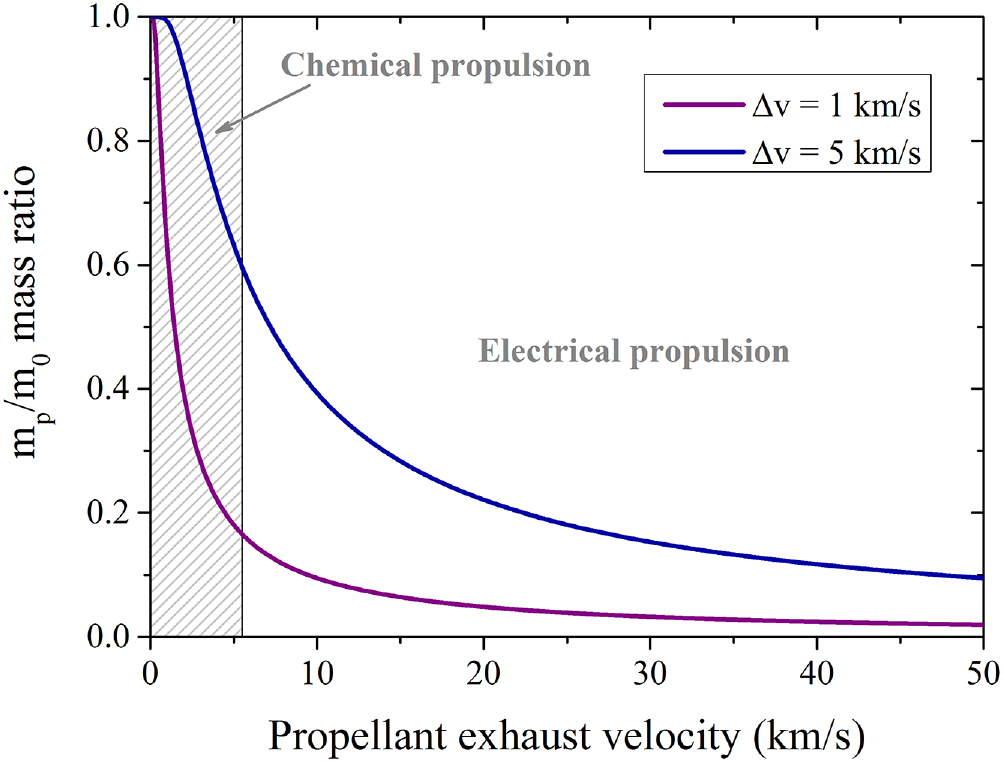
\includegraphics[width=0.7\linewidth]{img/introduction/mass_ratio_vs_exhaust_velocity}
	\caption{Ratio of the propellant mass to the initial mass as a function of the exhaust velocity ve for two values of the velocity increment $\Delta v$ . The dashed area corresponds to the domain of chemical propulsion with ve below 5.5 $km \, s^{-1}$. \cite{mazouffre_electric_2016} }
	\label{fig:massratiovsexhaustvelocity}
\end{figure}



\section{Magnetic Nozzle}
Magnetic nozzle is a convergent-divergent magnetic field that guides, expands and accelerates a plasma jet into vacuum for the purpose of space propulsion. \cite{andersen_continuous_1969,boswell_experimental_2004,williams_fusion_2003} The configuration is of the magnetic field in the magnetic nozzle plays a similar role to the walls of a Laval nozzle, see Fig. \ref{fig:magnetic-nozzle}. The plasma flow starts from subsonic at one end can be accelerated to supersonic at the other end. 

One advantage of magnetic nozzle is that it can operate contactlessly. Since the magnetic nozzle converts the plasma thermal energy into kinetic energy, so the thrust and specific impulse are strongly dependent on the temperature of the plasma flow. Higher the plasma temperature, more effective the plasma thruster. The magnetic field in the magnetic nozzle bounds the hot plasma, and therefore prevents the contact of the nozzle wall and the hot plasma jet. Hence, magnetic nozzle is an appealing plasma acceleration technology. Fig. \ref{fig:massratiovsexhaustvelocity} shows the comparison between magnetic nozzle and traditional chemical rocket.

Moreover, the configuration of magnetic field in magnetic nozzle is important for many other applications,\cite{smolyakov_quasineutral_2021} such as the magnetic divertors in fusion devices,\cite{ryutov_divertor_2016,togo_characteristics_2019} and is also related to the solar wind and accretion flow.\cite{jockers_stability_1968,aikawa_stability_1979} 

\begin{figure}[H]
	\centering
	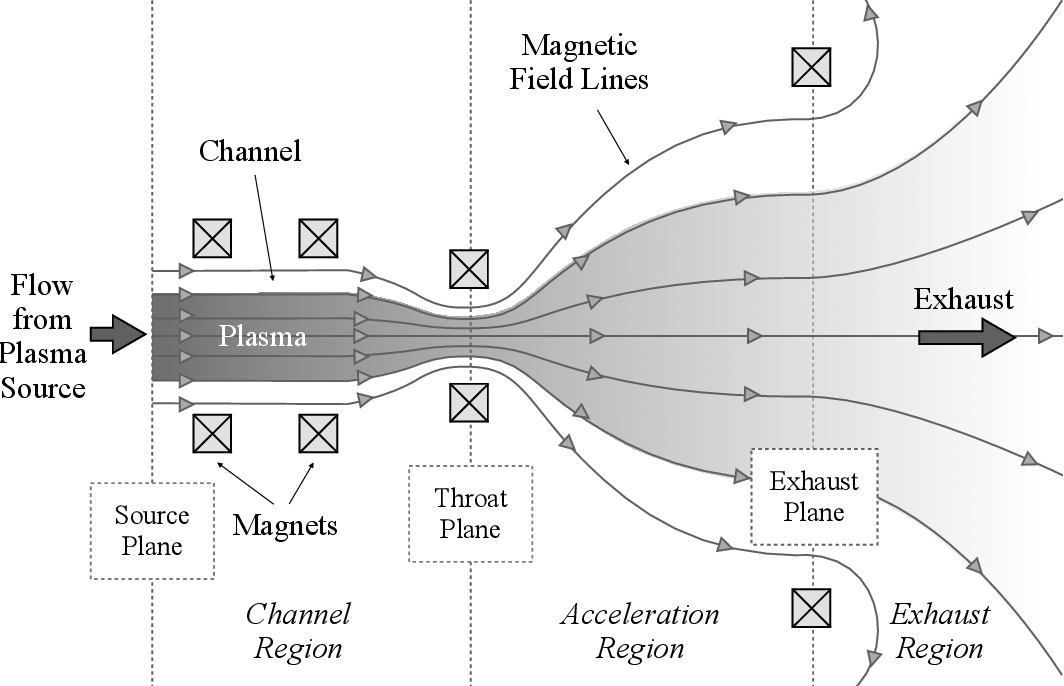
\includegraphics[width=0.7\linewidth]{img/introduction/magnetic_nozzle}
	\caption{Example of a magnetic nozzle configuration. In our models, we define the magnetic nozzle as the region downstream from the throat plane, which can be further divided into an acceleration region and exhaust region. The channel connects the plasma source (not shown) with the magnetic nozzle. \cite{little_performance_2015}}
	\label{fig:magnetic-nozzle}
\end{figure}


\section{Plasma Instability}
However, the plasma motion is determined by the Lorentz force, the nature of the nonlinearity of the motion makes it hard to predict analytically. Since the construction of Tokamak, people underestimated the difficulty of describing plasma motion. Hence, in order to maintain the equilibrium in the Tokamak, people start analyzing the stability of plasma. Nowadays, the study of plasma instabilities is an important area in plasma physics. 

Consider a plasma system in at equilibrium, we introduce a small perturbation to it. The stability of the system determines if the perturbations will grow, oscillate, or be damped out. Similar to the study of mechanical stability at equilibrium. See Fig. \ref{fig:stability-visualization}.

\begin{figure}[H]
	\centering
	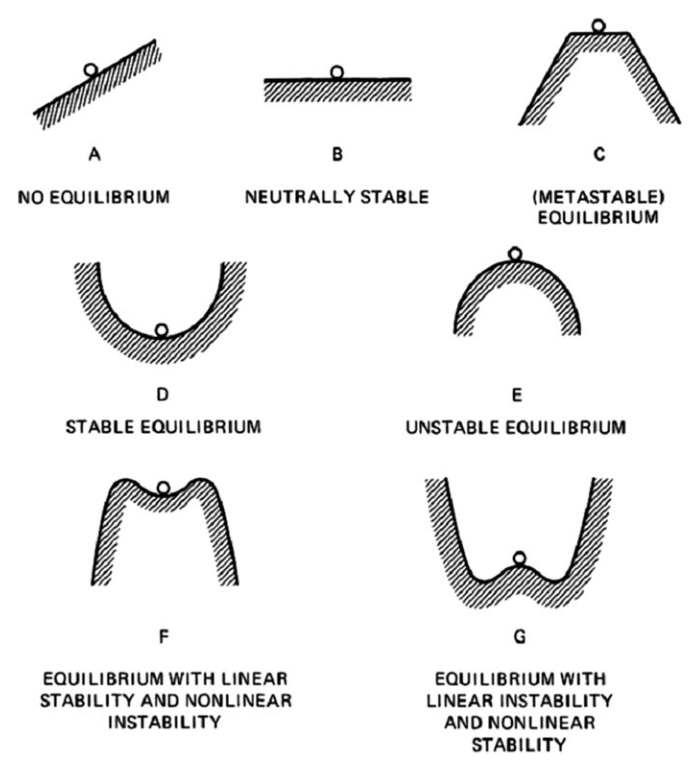
\includegraphics[width=0.7\linewidth]{img/introduction/stability_visualization}
	\caption{Mechanical analogy of various types of equilibrium. \cite{chen_introduction_2016}}
	\label{fig:stability-visualization}
\end{figure}


\subsection{Illustration: Two-Stream Instability}
We take the famous two-stream instability as an illustration. Let the plasma be cold ($k_BT_e = k_BT_i = 0$), let there be no magnetic field ($B_0=0$). The linearized continuity equations are
\begin{align} 
	\pdv{n_{i1}}{t} + n_0\pdv{v_{i1}}{x} &= 0  \label{eq:two-stream-continuity1} \\
	\pdv{n_{e1}}{t} + n_0\pdv{v_{e1}}{x} + v0\pdv{n_{e1}}{x} &= 0 \label{eq:two-stream-continuity2}
\end{align}

And the linearized equations of motion are
\begin{align} 
	Mn_0\pdv{v_{i1}}{t} &= en_0E_1  \label{eq:two-stream-eom1} \\
	mn_0\left(\pdv{v_{e1}}{t} + v_0\pdv{v_{e1}}{x}\right) &= -en_0E_1 \label{eq:two-stream-eom2}
\end{align}
Here $v_0$ is the velocity of electron respect to the ions (the ion velocity at equilibrium is taken to be $v_{i0}=0$), $n_0$ is the equilibrium density of both ion and electron, $v_{i1}$ and $v_{e1}$ are perturbed velocity of ions and electrons, and $E_1$ is the perturbed electron field.

If we assume perturbed electric field takes the wave form
\[ E_1 = E\exp(i(kx-\omega t)) \]
Plug this perturbed electric field into Eq.(\ref{eq:two-stream-eom1}) and (\ref{eq:two-stream-eom2}), then we can solve for $v_{i1}$ and $v_{e1}$,
\begin{align*}
	v_{i1} &= \frac{ie}{M\omega} E \\
	v_{e1} &= -\frac{ie}{m}\frac{E}{\omega-kv_0}
\end{align*}

Using the perturbed velocities, the continuity equations Eq.(\ref{eq:two-stream-continuity1}) and (\ref{eq:two-stream-continuity2}) yields
\begin{align*}
	n_{i1} &= \frac{ien_0k}{M\omega^2} E \\
	n_{e1} &= \frac{iekn_0}{m(\omega-kv_0)^2}E
\end{align*}

Finally, plug them into the Poisson's equation
\[ \epsilon_0 \pdv{E_1}{x} = e(n_{i1}-n_{e1}) \]
We now have the dispersion relation
\[ 1 = \omega_p \left[\frac{m/M}{\omega^2}+\frac{1}{(\omega-kv_0)^2}\right] \]

Solving this equation for $\omega$, there is chance we will get complex frequency,
\[ \omega = \omega_r + i\omega_i \]
where $\omega_r, \omega_i \in\mathbb{R}$. Then the perturbed electric field becomes
\[ E_1 = E\exp(i(kx-\omega_rt))\exp(\omega_it) \]

When $\omega_i < 0$, it is a damped wave, when $\omega_i > 0$, it grows exponentially and therefore unstable. Since the complex root comes with pair, as long as $\omega_i\neq 0$, one of the roots must correspond to an unstable wave. The following graph shows the two-stream instability in phase space.

\begin{figure}[H]
	\centering
	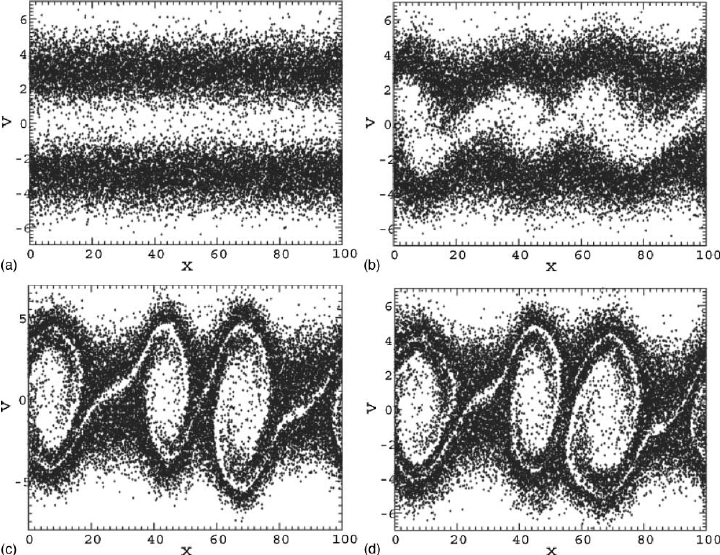
\includegraphics[width=0.7\linewidth]{img/introduction/two_stream_instability}
	\caption{Visualization of two-stream instability in the phase space. (a) Initially the ion and electron flow are in opposite direction. (b) The velocity of both flows start to oscillate. (c) Chaotic behavior occurs. (d) The chaotic behavior continues. \cite{ha_nonlinear_2011}}
	\label{fig:two_stream_instability}
\end{figure}

\subsection{Stability of Configurations Similar to Magnetic Nozzle}
Accretion flow has configuration similar to the magnetic nozzle. It is natural to find studies of stability the accretion flow. However, the results are still debatable. \cite{keto_stability_2020,aikawa_stability_1979,stellingwerf_stability_1978}


\section{Goals of this Thesis}
The goals of this thesis is to first study the spectral method for solving the instability problem. When using the spectral method, it is necessary to understand different discretizations of the operators, such as finite difference, finite element and DVR method.

Once the spectral method is introduced, we can use it to study the instability of plasma in magnetic nozzle. We can use different discretization techniques, and compare the results from different methods.

Finally, we need to take care of the filtering of the spectral pollution.


\section{Thesis Outline}
The theory of spectral methods will be discussed in chapter \ref{chap:spectral_method}. In this chapter, different discretiation methods will be introduced. Moreover, a very important concept, spectral pollution, will be introduced in detailed in the final section of this chapter.

Then, in chapter \ref{chap:governing_equations} is the discussion of governing equations and its linearization. The formulation of the problem will be derived in this chapter.

In chapter ??, we ill use the equations derived in chapter \ref{chap:governing_equations} to conduct numerical experiments. The goal is to investigate the frequency of each modes. The filtering methods of spurious modes will be introduced.

Conclusion will in chapter ??


\section{Spectral Method}
\begin{frame}{Spectral Method}
  Eq.(\ref{eq:polynomial_eigenvalue_problem}) can be reformulate as 
  \begin{equation} \label{eq:eigenvalue-problem}
	\mqty[ 0 & 1\\ \hat{M} & \hat{N} ]\mqty[ \tilde{v}\\ \omega \tilde{v}] = \omega\mqty[ \tilde{v}\\ \omega \tilde{v}]
\end{equation}
where the operators $\hat{M}$ and $\hat{N}$ are defined as
\begin{align*}
	\hat{M} = &-\left[(1-v_0^2)\pdv[2]{}{z} 
	-\left(3v_0 + \frac{1}{v_0}\right)\pdv{v_0}{z}\pdv{}{z}\right. \\ 
  &- \left.  \left(1-\frac{1}{v_0^2}\right)\left(\pdv{v_0}{z}\right)^2 
	- \left(v_0+\frac{1}{v_0}\right)\pdv[2]{v_0}{z}\right] \\
	\hat{N} = &-2i\left(v_0\pdv{}{z} +\pdv{v_0}{z} \right) 
\end{align*}
  Then by discretizing operators $\hat{M},\hat{N}$, this becomes an algebraic eigenvalue problem.
\end{frame}

\begin{frame}{Spectral Pollution}
  \begin{itemize}
    \item All modes of Eq.(\ref{eq:polynomial_eigenvalue_problem}) with $v_0=\text{const}$ are stable.
    \item Yet all discretization show unstable modes.
  \end{itemize}
  \begin{figure}[htbp]	
    \centering
    \begin{subfigure}[b]{0.5\linewidth}
      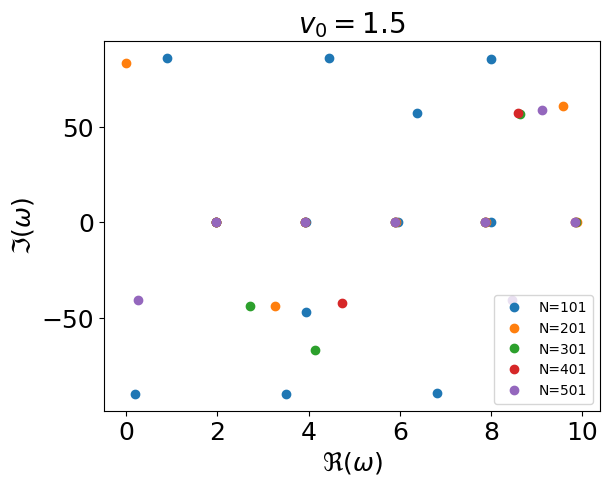
\includegraphics[width=0.9\linewidth]{figures/eigvals-bad} 
      \caption{Unfiltered eigenvalues.}
    \end{subfigure}%
    \begin{subfigure}[b]{0.5\linewidth}
      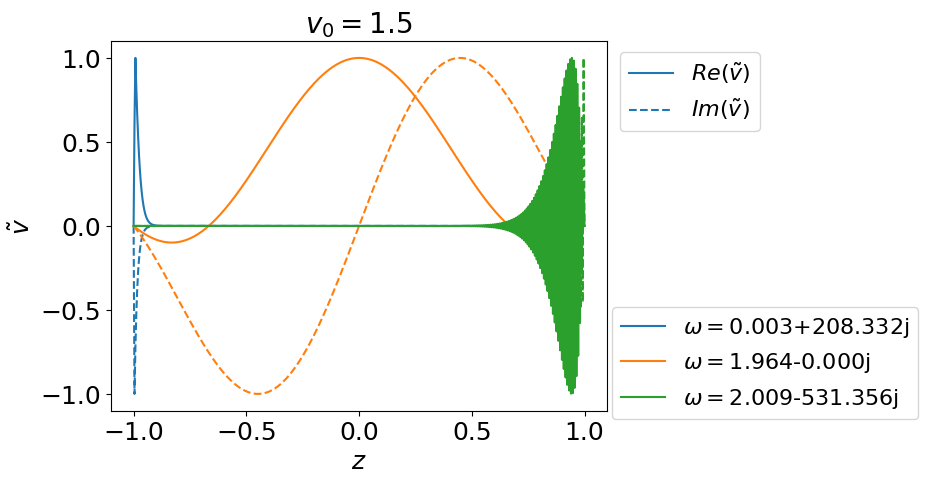
\includegraphics[width=0.9\linewidth]{figures/eigvecs-bad} 
      \caption{First few unfiltered eigenfunctions.}
    \end{subfigure}
    \caption{Finite difference discretization was used. Spurious modes occurs regardless of the resolution.}
    \label{fig:results-bad}
  \end{figure}
\end{frame}

\begin{frame}{Filtering Spurious Modes}
  \begin{figure}[htbp]
    \centering
    \begin{subfigure}[b]{0.5\linewidth}
      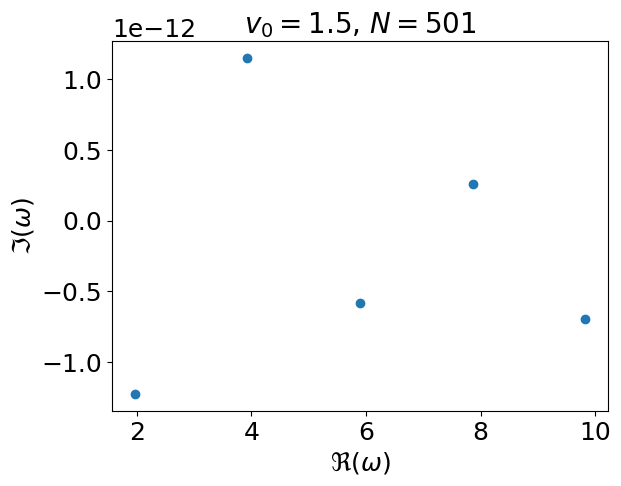
\includegraphics[width=\linewidth]{figures/eigvals-good} 
      \caption{Filtered eigenvalues.}
    \end{subfigure}%
    \begin{subfigure}[b]{0.5\linewidth}
      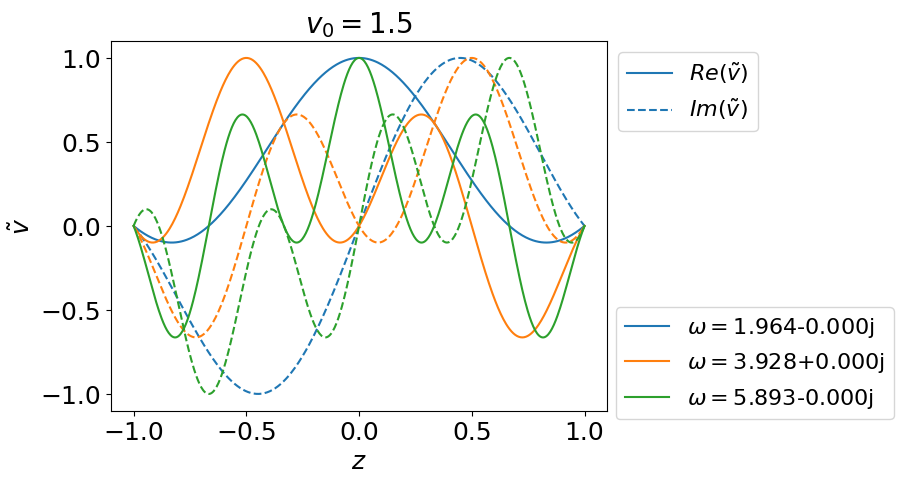
\includegraphics[width=\linewidth]{figures/eigvecs-good} 
      \caption{First few filtered eigenfunctions.}
    \end{subfigure}
    \caption{The spurious modes are changing under different resolution. We can filter them by convergence test.}
    \label{fig:results-good}
  \end{figure}
\end{frame}

\section{Governing Equations}
\begin{frame}{Governing Equations}
  For convenience, we nondimensionalize the governing equations by normalizing the velocity to $c_s$, $v\mapsto v/c_s$, $z$ to system length $L$, coordinate along the nozzle $z \mapsto z/L$ and time $t\mapsto c_s t/L$. The governing equations become
  \begin{align}
    & \text{Cons. of Den.}  &&\pdv{n}{t} + n\pdv{v}{z} + v\pdv{n}{z} - nv\frac{\partial_z B}{B} = 0 \\
    & \text{Cons. of Mom.}  &&n\pdv{v}{t} + nv\pdv{v}{z} = -\pdv{n}{z}
  \end{align}
  where $n$ is nondimensionalized density. 

  The nondimensionalized equilibrium condition is
  \begin{align}
      &\pdv{z}(\frac{n_0v_0}{B}) = 0 \label{eq:equilibrium-convervation-of-mass}\\
      &v_0\pdv{v_0}{z} = -\frac{1}{n_0}\pdv{n_0}{z} \label{eq:equilibrium-convervation-of-momentum}
  \end{align}
  where $n_0$ and $v_0$ are equilibrium density and velocity, respectively.
\end{frame}

\begin{frame}{Linearized Equations}
  To linearized the governing equations, we perturbed the density and velocity profiles. Let $n = n_0(z) + \tilde{n}(z,t)$ and $v = v_0(z) + \tilde{v}(z,t)$, where $\tilde{n}$ and $\tilde{v}$ are small perturbed quantities. Then Eq.(\ref{eq:equilibrium-convervation-of-mass}) and Eq.(\ref{eq:equilibrium-convervation-of-momentum}) becomes 
  \begin{align}
    &\frac{1}{n_0}\pdv{\tilde{n}}{t} 
    + \pdv{\tilde{v}}{z} + v_0\tilde{Y} + \tilde{v}\frac{\partial_z n_0}{n_0} - \tilde{v}\frac{\partial_z B}{B} = 0 
    \label{eq:linearized-conservation-of-mass}
    \\
    &\pdv{\tilde{v}}{t} + \pdv{(v_0\tilde{v})}{z} = -\tilde{Y}
    \label{eq:linearized-conservation-of-momentum}
  \end{align}
  where 
  \[ \tilde{Y} \equiv \frac{1}{n_0}\pdv{\tilde{n}}{z} - \frac{\partial_z n_0}{n_0^2}\tilde{n} = \pdv{z}(\frac{\tilde{n}}{n_0}) \]
\end{frame}
 
\begin{frame}{Polynomial Eigenvalue Problem}
  Suppose the perturbed quantities are oscillating, $\tilde{n}\sim \exp(-i\omega t)$ and $\tilde{v} \sim \exp(-i\omega t)$. The perturbed quantities will blow up if $\Im(\omega) > 0$, so-called unstable flow. 

  Substituting them into Eq.(\ref{eq:linearized-conservation-of-mass}) and Eq.(\ref{eq:linearized-conservation-of-momentum}), and combine the two equation, we get the so-called polynomial eigenvalue problem
  \begin{equation}
    \begin{aligned}
      &\omega^2 \tilde{v} \\ 
      +& 2i\omega\left(v_0\pdv{}{z} + \pdv{v_0}{z}\right) \tilde{v} \\
      +& \left[ (1-v_0^2)\pdv[2]{}{z} 
        -\left(3v_0 + \frac{1}{v_0}\right)\pdv{v_0}{z}\pdv{}{z} \right. \\
        &- \left. \left(1-\frac{1}{v_0^2}\right)\left(\pdv{v_0}{z}\right)^2 
      - \left(v_0+\frac{1}{v_0}\right)\pdv[2]{v_0}{z} \right]\tilde{v}
      = 0
    \end{aligned}
    \label{eq:polynomial_eigenvalue_problem}
  \end{equation}
\end{frame}

\chapter{Theoretical Analysis} \label{chap:theoretical-analysis}
In order to determine the best tool to tackle the problem. We need to first simplify the problem.

\section{Fluid Description for Flow}
In this section, we will derive the governing equations of the flow in magnetic nozzle, starting from the fluid description for plasma.

We start by deriving the usefule form of the conservation of density,
\[ \pdv{n}{t} + \div(n\mathbf{v}) = 0 \]
where $\mathbf{v}$ here denotes the fluid velocity of the plasma flow.

We can get the fluid velocity by taking the integral
\[ \mathbf{v} = \frac{1}{n}\int_{\mathbb{R}^3} \mathbf{v}_p f(\mathbf{x}, \mathbf{v}_p, t) d^3\mathbf{v}_p \]

Denote the particle velcity as $\mathbf{v}_p$, we can decompose the particle velocity vector as $\mathbf{v}_p = (v_\parallel,v_\perp)$, where $v_\parallel$ and $v_\perp$ are the magnitudes of components that are parallel to and perpendicular to the magnetic field line, respectively. Due to the Lorentz force, the charged particles gyrates about the magnetic field lines, see Fig.\ref{fig:gyrate-along-b-field}. Hence, the $v_\perp$ will be averaged to zero the expression for plasma fluid velocity can be simplied as
\[\mathbf{v} = v\mathbf{B}/B\]
where $v$ is the fluid speed along the magnetic field lines. This makes sence because the charged particles flows along $\mathbf{B}$.

By expanding the divergence term, and using the divergence free condition $\div B=0$, we have
\[ \pdv{n}{t} + \mathbf{B}\cdot \grad(\frac{nv}{B}) = 0 \]
Since the magnetic field lines are aligned with the central axis of the nozzle, which we denote as z-axis, so $\mathbf{B} = B\hat{z}$. Now we obtain the conservation of density for the magnetic nozzle,
\begin{equation}
	\pdv{n}{t} + B\pdv{z}(\frac{nv}{B}) = 0
\end{equation}

The second governing equation is the conservation of momentum,
\[ mn\pdv{\mathbf{v}}{t} + mn\mathbf{v}\cdot\grad\mathbf{v} = -\grad p \]
where $m$ is the ion mass. This equation tells us the plasma flow is driven by pressure.

The equation of state is given by the isothermal condition,
\begin{equation} \label{eq:eos}
	p = nk_BT
\end{equation}
There are two main reasons. First the plasma particles are confined to the magnetic field lines. This reduces the particle collisions and energy exchanges. Moreover, the electrons have high mobility, they will quickly fill up any charge cavities and thus maintain a constant temperature. Hence, we can safely assume the plasma flow is isothermal.

Therefore, we have
\begin{equation}
	\pdv{v}{t} + v\pdv{v}{z} = -c_s^2\frac{1}{n}\pdv{n}{z}
\end{equation}
where $c_s^2 = k_BT/m$ is the square of sound speed.

Therefore, the dynamics of the plasma flow in magnetic nozzle can be characterized by the conservation of density and momentum,
\begin{align*}
	 & \pdv{n}{t} + B\pdv{z}(\frac{nv}{B}) = 0                \\
	 & \pdv{v}{t} + v\pdv{v}{z} = -c_s^2\frac{1}{n}\pdv{n}{z}
\end{align*}
The magnetic field profile was discussed in Sec.\ref{sec:magnetic-field-in-nozzle}.

In this research, we are interested in the stability of the equilibrium flow in the nozzle. Let's denote $n_0$ and $v_0$ as equilibrium density and equilibrium velocity, respectively. Since they are stationary (time independent) solutions to the above set of equations, so they satisfy the so-called equilibrium condition,
\begin{align*}
	 & B\pdv{z}(\frac{n_0v_0}{B})  = 0                   \\
	 & v_0\pdv{v_0}{z} = -c_s^2\frac{1}{n_0}\pdv{n_0}{z}
\end{align*}

\section{Non-dimensionalization}
For convenience, we nondimensionalize the governing equations by normalizing the velocity to $c_s$, $v\mapsto v/c_s$, $z$ to system length $L$, $z \mapsto z/L$ and time $t\mapsto c_s t/L$. The governing equations become
\begin{align}
	 & \pdv{n}{t} + n\pdv{v}{z} + v\pdv{n}{z} - nv\frac{\partial_z B}{B} = 0
	\label{eq:conservation-of-density}
	\\
	 & n\pdv{v}{t} + nv\pdv{v}{z} = -\pdv{n}{z}
	\label{eq:conservation-of-momentum}
\end{align}
and the nondimensionalized equilibrium condition is
\begin{align}
	 & \pdv{z}(\frac{n_0v_0}{B}) = 0 \label{eq:equilibrium-conservation-of-density}                 \\
	 & v_0\pdv{v_0}{z} = -\frac{1}{n_0}\pdv{n_0}{z} \label{eq:equilibrium-conservation-of-momentum}
\end{align}

\section{Velocity Profiles at Equilibrium}
In this section we will solve the equilibrium velocity profile, $v_0$, from the nondimensionalized equilibrium condition, Eq.(\ref{eq:equilibrium-conservation-of-density}) and Eq.(\ref{eq:equilibrium-conservation-of-momentum}).
We start by substituting $\frac{1}{n_0}\pdv*{n_0}{z}$ into Eq.(\ref{eq:equilibrium-conservation-of-density}), then it becomes
\[ (v_0^2-1)\pdv{v_0}{z} = -\frac{v_0}{B}\pdv{B}{z} \]

Notice that there is a singularity at $v_0=1$, the sonic speed.

This is a separable equation, integrate it and use the conditions at midpoint $B(0)=B_m, v_0(0)=v_m$ we get
\[ v_0^2e^{-v_0^2} = \frac{B^2}{B_m^2}v_m^2e^{-v_m^2} \]
We can now express $v_0$ using the Lambert W function (see Appendix \ref{app:lambert-w}),
\[ v_0(z) = \left[ -W_k\left(-\frac{B(z)^2}{B_m^2}v_m^2e^{-v_m^2}\right) \right]^{1/2} \]
where the subscript $k$ of $W$ stands for branch of Lambert W function.

When considering the velocity profile of a nozzle flow, various scenarios can be distinguished based on the Mach number parameter ($v_m$) and the branch ($k$) used in the expression for the Mach number distribution, denoted as $v_0(z)$. These parameters play a crucial role in determining the flow characteristics. The selection of appropriate $v_m$ and $k$ values facilitates the control of the flow characteristics in the nozzle, allowing for the realization of various flow regimes, such as subsonic, supersonic, transonic, accelerating, or decelerating profiles. Different velocity profiles are shown in Fig.\ref{fig:velocity-profiles}.

Firstly, for the case where $v_m < 1$ and $k = 0$, the resulting velocity profile is classified as subsonic. This means that both at the entrance and exit of the nozzle, the velocity remains subsonic, and the midpoint velocity is also less than unity ($v_m < 1$). A subsonic flow is characterized by fluid velocities that are slower than the local speed of sound.

On the other hand, when $v_m > 1$ and $k = -1$, the velocity profile corresponds to a supersonic flow regime. In this situation, the fluid velocities at both the entrance and exit of the nozzle are supersonic, and the midpoint velocity ($v_m$) exceeds the value of unity ($v_m > 1$). Supersonic flow is characterized by velocities that surpass the speed of sound.

Furthermore, when $v_m = 1$, the velocity profile becomes transonic. In this case, the midpoint velocity is exactly at the sonic threshold ($v_m = 1$), where the fluid velocity equals the local speed of sound. Transonic flows often exhibit a combination of subsonic and supersonic regions, and this regime poses unique challenges due to the presence of singularity at the nozzle throat. We will discuss this thoroughly in Chap.\ref{chap:singular-perturbation}.

To achieve an accelerating velocity profile, a configuration with $k = 0$ for $x < 0$ and $k = -1$ for $x > 0$ is employed. Here, $x$ represents the spatial coordinate along the nozzle length. With this setup, the flow starts subsonically and gradually accelerates to a supersonic speed as it propagates along the nozzle.

Conversely, a decelerating velocity profile can be obtained by adopting a similar approach but with reversed values of $k$. Specifically, the configuration will have $k = -1$ for $x < 0$ and $k = 0$ for $x > 0$, causing the flow to start supersonically and decelerate to subsonic velocities further down the nozzle.

\begin{figure}[H]
	\centering
	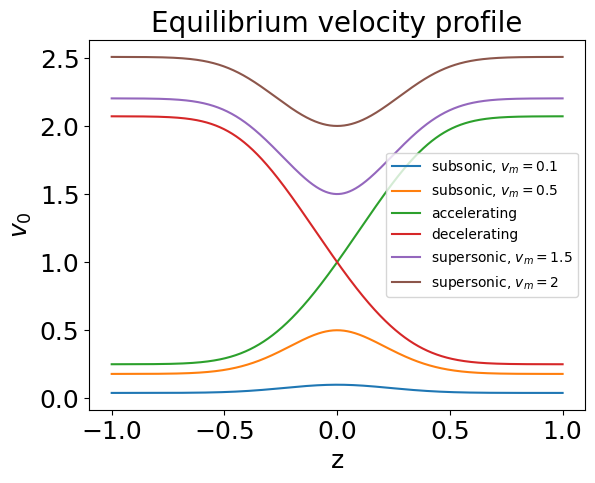
\includegraphics[width=0.7\linewidth]{img/velocity-profiles}
	\caption{The velocity profile in the magnetic nozzle is completely determined by the midpoint mach number $v_m$ and the branch $k$. A subsonic profile can be obtained by selecting $v_m<1$ and $k=0$. On the other hand, a supersonic profile can be obtained by setting $v_m>1$ and $k=-1$. Lastly, for the transonic velocity profiles, the midpoint velocity is set to unity, $v_m=1$, and then by choose $k=0$ for $x<0$ and $k=-1$ for $x>0$ we get accelerating profile. Decelerating profile can be obtained similarly.}
	\label{fig:velocity-profiles}
\end{figure}

\section{Linearized Governing Equations}
As illustrated in Sec.\ref{sec:two-stream-instability}, it is essential to linearize the governing equations in order to investigate the instability of plasma. Now we are going to derive the linearized governing equations with the equilibrium conditions given in above.

Let $n = n_0(z) + \tilde{n}(z,t)$ and $v = v_0(z) + \tilde{v}(z,t)$, where $\tilde{n}$ and $\tilde{v}$ are small perturbed quantities.

We first linearize Eq.(\ref{eq:conservation-of-density}) by setting $n=n_0+\tilde{n}$ and $v=v_0+\tilde{v}$,
\[    \pdv{(n_0+\tilde{n})}{t}
	+ (n_0+\tilde{n})\pdv{(v_0+\tilde{v})}{z}
	+ (v_0+\tilde{v})\pdv{(n_0+\tilde{n})}{z}
	- (n_0+\tilde{n})(v_0+\tilde{v})\frac{\partial_z B}{B} = 0
\]
By ignoring the second order perturbations, we obtain
\[ \frac{1}{n_0}\pdv{\tilde{n}}{t}
	+ \pdv{v_0}{z} + \frac{\tilde{n}}{n_0}\pdv{v_0}{z} + \pdv{\tilde{v}}{z}
	+ \frac{v_0}{n_0}\pdv{n_0}{z} + \frac{\tilde{v}}{n_0}\pdv{n_0}{z} + \frac{v_0}{n_0}\pdv{\tilde{n}}{z}
	- v_0\frac{\partial_z B}{B} - \tilde{v}\frac{\partial_z B}{B} - \tilde{n}\frac{v_0}{n_0}\frac{\partial_z B}{B} = 0
\]


Using the equilibrium condition Eq.(\ref{eq:equilibrium-conservation-of-density}), some of the terms are canceled. Moreover, the last term can be written as
\[ \tilde{n}\frac{v_0}{n_0}\frac{\partial_z B}{B} = \frac{\tilde{n}}{n_0}\left( \frac{\partial_z n_0}{n_0}v_0 + \pdv{v_0}{z} \right) \]
Now, we get the linearized conservation of mass,
\begin{equation} \label{eq:linearized-conservation-of-density}
	\frac{1}{n_0}\pdv{\tilde{n}}{t}
	+ \pdv{\tilde{v}}{z} + v_0\tilde{Y} + \tilde{v}\frac{\partial_z n_0}{n_0} - \tilde{v}\frac{\partial_z B}{B} = 0
\end{equation}
where
\[ \tilde{Y} \equiv \frac{1}{n_0}\pdv{\tilde{n}}{z} - \frac{\partial_z n_0}{n_0^2}\tilde{n} = \pdv{z}(\frac{\tilde{n}}{n_0}) \]

To linearize the conservation of momentum, we follow the same logic by substituting $n=n_0+\tilde{n}$, and $v=v_0+\tilde{v}$ in Eq.(\ref{eq:conservation-of-momentum}),
\[ (n_0+\tilde{n})\pdv{(v_0+\tilde{v})}{t} + (n_0+\tilde{n})(v_0+\tilde{v})\pdv{(v_0+\tilde{v})}{z} = -\pdv{n}{z} \]

Again, ignore second order perturbations and rearange terms, we have
\[ \pdv{v_0}{t} + v_0\pdv{v_0}{z} + \tilde{v}\pdv{v_0}{z}
	= -\frac{1}{n_0}\pdv{n_0}{z} -\frac{1}{n_0}\pdv{\tilde{n}}{z} -v_0\frac{v_0}{z} - \frac{\tilde{n}}{n_0}v_0\pdv{v_0}{z} \]
Using the equilibrium condition Eq.(\ref{eq:equilibrium-conservation-of-momentum}) on the RHS, we get the linearized conservation of momentum,
\begin{equation} \label{eq:linearized-conservation-of-momentum}
	\pdv{\tilde{v}}{t} + \pdv{(v_0\tilde{v})}{z} = -\tilde{Y}
\end{equation}

\section{Polynomial Eigenvalue Problem}
We can further simplify the problem by combining Eq.(\ref{eq:linearized-conservation-of-density}) and Eq.(\ref{eq:linearized-conservation-of-momentum}) into a single equation. We can substitute Eq.(\ref{eq:linearized-conservation-of-momentum}) into Eq.(\ref{eq:linearized-conservation-of-density}) to eliminate $\tilde{Y}$,

\begin{equation} \label{eq:single-governing-equation}
	\pdv{t}\frac{\tilde{n}}{n_0}
	+ \pdv{\tilde{v}}{z} - v_0\left(\pdv{t}\tilde{v}
	+ \pdv{(v_0\tilde{v})}{z}\right)
	+ \tilde{v}\frac{\partial_z n_0}{n_0}
	- \tilde{v}\frac{\partial_z B}{B}
	= 0
\end{equation}

In order to investigate the instability of the flow, we need formulate it as an eigenvalue problem. To do that, we assume the perturbed density and velocity are oscillatory, i.e. $\tilde{n}, \tilde{v} \sim \exp(-i\omega t)$, where $\omega$ is the oscillation frequency of the perturbed quantities. This frequency can be a complex number.

As illustrated in Sec.\ref{sec:two-stream-instability}, the flow can be stable or unstable depending on the imaginary part of the frequency. If $\Im(\omega) > 0$, then the perturbed quantities $\tilde{n} \sim \exp(\Im(\omega) t)$, which means it grows exponentially with time, hence unstable. If $\Im(\omega) \leq 0$, then the amplitude of the perturbed quanties are either unchanged or exponentially decreasing, hence the flow is stable.

By assuming oscillatory perturbed quantities, Eq.(\ref{eq:single-governing-equation}) becomes,
\begin{equation}
	-i\omega\frac{\tilde{n}}{n_0}
	+ \pdv{\tilde{v}}{z} - v_0\left(-i\omega\tilde{v}
	+ \pdv{(v_0\tilde{v})}{z}\right)
	+ \tilde{v}\frac{\partial_z n_0}{n_0}
	- \tilde{v}\frac{\partial_z B}{B}
	= 0
\end{equation}

Using the equilibrium condition Eq.(\ref{eq:equilibrium-conservation-of-density}), we can eliminate the term $\partial_z B/B$,
\[
	-i\omega\frac{\tilde{n}}{n_0}
	+ \pdv{\tilde{v}}{z}
	+ v_0\left(i\omega \tilde{v} - v_0\pdv{\tilde{v}}{z} - \tilde{v}\pdv{v_0}{z} \right)
	- \tilde{v}\frac{\partial_z v_0}{v_0}
	= 0
\]

Rearrange terms, we have
\[
	-i\omega\frac{\tilde{n}}{n_0}
	+ i\omega v_0\tilde{v}
	+ (1-v_0^2)\pdv{\tilde{v}}{z}
	- \left(v_0+\frac{1}{v_0}\right)\pdv{v_0}{z}\tilde{v} = 0
\]

Now we take $\pdv*{t}$ on Eq.(\ref{eq:linearized-conservation-of-momentum}). Recall the fact that $\tilde{Y} = \partial_z(\tilde{n}/n_0)$, we have
\[
	\omega^2\tilde{v} + i\omega\left(v_0\pdv{\tilde{v}}{z} + \tilde{v}\pdv{v_0}{z}\right)
	= \pdv{t}\pdv{z}(\frac{\tilde{n}}{n_0})
\]
Apply $\partial_t$ operator first, we get
\[
	\omega^2\tilde{v} + i\omega\left(v_0\pdv{\tilde{v}}{z} + \tilde{v}\pdv{v_0}{fz}\right)
	= \pdv{z}(-i\omega v_0\tilde{v}
	- (1-v_0^2)\pdv{\tilde{v}}{z}
	+ \left(v_0+\frac{1}{v_0}\right)\pdv{v_0}{z}\tilde{v})
\]
Expand the RHS and collect terms, we get
\begin{equation} \label{eq:polynomial-eigenvalue-problem}
	\begin{aligned}
		 & \omega^2 \tilde{v}                                          \\
		 & +2i\omega\left(v_0\pdv{}{z} + \pdv{v_0}{z}\right) \tilde{v} \\
		 & +\left[ (1-v_0^2)\pdv[2]{}{z}
			-\left(3v_0 + \frac{1}{v_0}\right)\pdv{v_0}{z}\pdv{}{z}
			- \left(1-\frac{1}{v_0^2}\right)\left(\pdv{v_0}{z}\right)^2
			- \left(v_0+\frac{1}{v_0}\right)\pdv[2]{v_0}{z} \right]\tilde{v}
		= 0
	\end{aligned}
\end{equation}

In mathematical terms, Eq.(\ref{eq:polynomial-eigenvalue-problem}) is a polynomial eigenvalue problem, where $\omega$ is an eigenvalue to the problem, and the velocity perturbation $\tilde{v}$ is an eigenfunction associated with the eigenvalue $\omega$. In the later chapters we will discuss the methods to tackle this problem.

\section{Analytical Solutions to Constant Velocity Case}
In this section we are going to tackle the simplest case of the polynomial eigenvalue problem, Eq.(\ref{eq:polynomial-eigenvalue-problem}), the constant velocity case.

The constant velocity profile can be viewed as the limit of $v_0(z)$ as the spread of magnetic field goes to infinity, $\delta\to\infty$. As the parameter $\delta$ approaches infinity, the width of the magnetic field enlarges and eventually becomes flat. In other words, a constant magnetic field. We can easily see that the velocity profile $v_0(z)$ becomes a constant as well.

In the following subsections, we will solve Eq.(\ref{eq:polynomial-eigenvalue-problem}) with constant velocity under two sets of boundary conditions, Dirichlet and fixed-open boundary condition.

\subsection{Dirichlet Boundary}
If we set the velocity profile of the equilibrium flow to constant $v_0=\text{const}$, then Eq.(\ref{eq:polynomial-eigenvalue-problem}) becomes a simple boundary value problem with second order constant coefficients differential equation.

\begin{equation} \label{eq:constant-v-problem-dirichlet}
	\omega^2\tilde{v} + 2i\omega v_0\pdv{\tilde{v}}{z} + (1-v_0^2)\pdv[2]{\tilde{v}}{z} = 0
\end{equation}

We need two boundary values in order to uniquely determine the solution (up to a constant). In this subsection, the so-called Dirichlet boundary condition will be used. It has the name because the function values are fixed at the two ends of the nozzle,
\[ \tilde{v}(-1) = \tilde{v}(1) = 0 \]
Since the left end, $z=-1$, is the entrance of the nozzle, we assume there is no perturbation at the entrance. As for the right end (exit of the nozzle), $z=1$, setting the velocity perturbation to 0 might not be the best boundary condition to describe the physical process of the plasma flow in the nozzle, it nevertheless serves as a starting point to the problem.

Now the solution to this problem is
\begin{equation} \label{eq:constant-v-solution-dirichlet}
	\tilde{v} = C\left[ \exp\left(i\omega\frac{z+1}{v_0+1}\right) - \exp\left(i\omega\frac{z+1}{v_0-1}\right) \right]
\end{equation}
where $C\in\mathbb{C}$ is a complex constant, and the frequencies are $\omega=n\pi(1-v_0^2)/2$ with $n\in\mathbb{Z}$.

This result tells us for constant velocity case, the flow in magnetic nozzle is stable regardless the velocity $v_0$. It is worth to mention $v_0=1$ is a singular point of this problem.

We will use this to benchmark the simulation results.

\begin{figure}[H]
	\centering
	\begin{subfigure}{0.5\textwidth}
		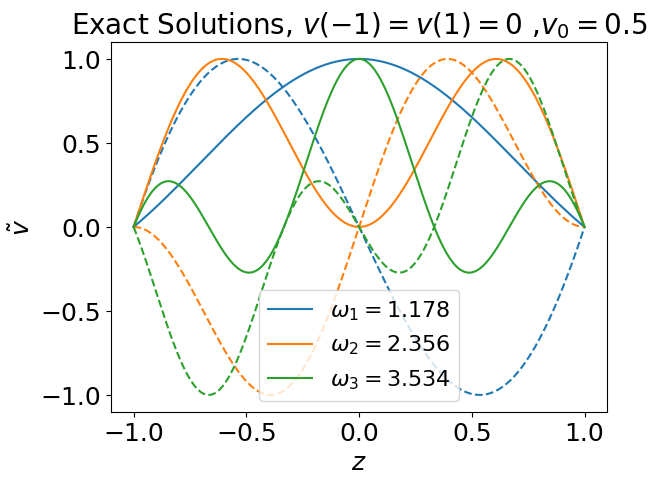
\includegraphics[width=\linewidth]{img/exact-fixed-fixed-v0=0.5}
		\caption{Subsonic}
	\end{subfigure}%
	\begin{subfigure}{0.5\textwidth}
		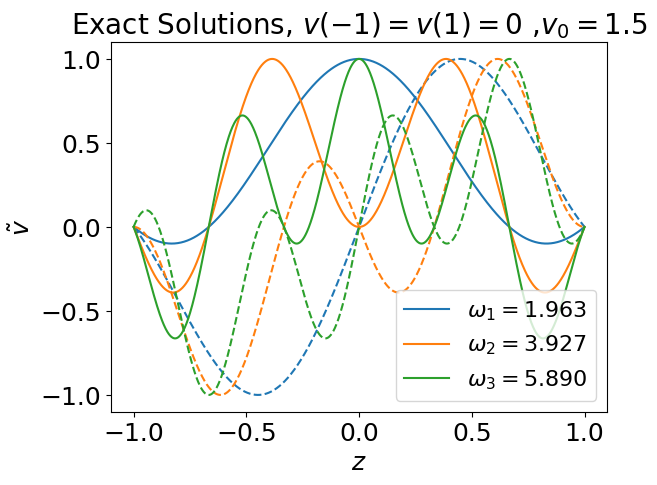
\includegraphics[width=\linewidth]{img/exact-fixed-fixed-v0=1.5}
		\caption{Supersonic}
	\end{subfigure}
	\caption{The plots show the first three non-zero exact solutions to Eq.(\ref{eq:constant-v-problem-dirichlet}) for both subsonic and supersonic case. These solutions are stable.}
	\label{fig:exact-v-dirichlet}
\end{figure}

\subsection{Fixed-Open Boundary}

\begin{equation} \label{eq:constant-v-problem-fixed-open}
	\omega^2\tilde{v} + 2i\omega v_0\pdv{\tilde{v}}{z} + (1-v_0^2)\pdv[2]{\tilde{v}}{z} = 0
	\quad
	\tilde{v}(-1) = \pdv{\tilde{v}}{z}\,(1) = 0
\end{equation}

The solution to this problem is
\begin{equation} \label{eq:constant-v-solution-fixed-open}
	\tilde{v} = \exp\left(i\omega\frac{z+1}{v_0+1}\right)
	- \exp\left(i\omega\frac{z+1}{v_0-1}\right)
\end{equation}
where $\omega = (v_0^2 - 1) \left[\frac{n\pi}{2} - \frac{1}{4}i\ln(\frac{v_0-1}{v_0+1})\right]$ with $n\in\mathbb{Z}$. The term $i\ln((v_0-1)/(v_0+1))\in\mathbb{C}$ and its imaginary part is positive for any $v_0\neq 1$. Therefore,
\begin{itemize}
	\item If $v_0<1$, then $\Im(\omega)<0$, it's damped oscillation, hence stable.
	\item If $v_0>1$, then $\Im(\omega)>0$, it's unstable.
\end{itemize}

Worth to mention, this is a very interesting solution with the following properties,
\begin{enumerate}
	\item The growth rate is independent the mode number $n$.
	\item The ground mode $n=0$ for subsonic case has non-zero real part and imaginary part.
\end{enumerate}

\begin{figure}[H]
	\centering
	\begin{subfigure}{0.5\textwidth}
		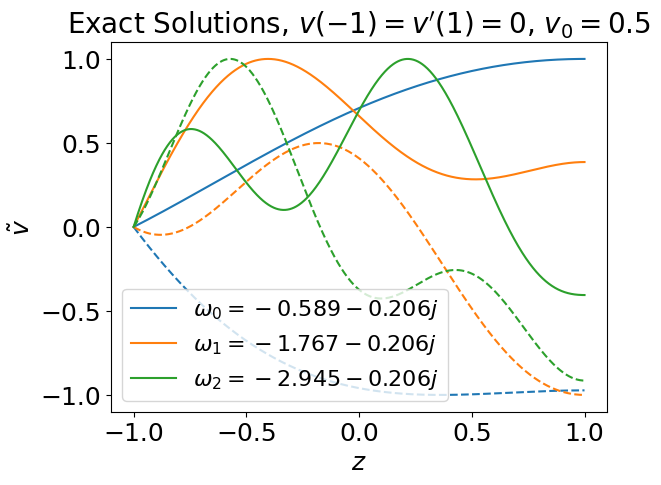
\includegraphics[width=\linewidth]{img/exact-fixed-open-v0=0.5}
		\caption{Subsonic, stable flow.}
	\end{subfigure}%
	\begin{subfigure}{0.5\textwidth}
		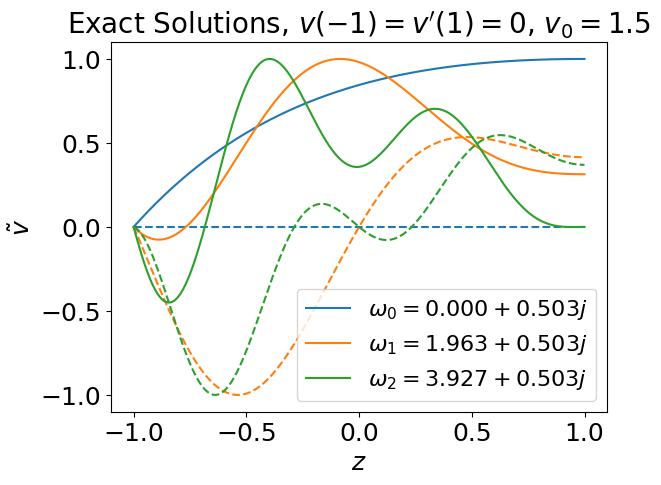
\includegraphics[width=\linewidth]{img/exact-fixed-open-v0=1.5}
		\caption{Supersonic, unstable flow.}
	\end{subfigure}
	\caption{The plots show the first three exact solutions to Eq.(\ref{eq:constant-v-problem-fixed-open}) for both subsonic and supersonic case. The flow is stable for subsonic case and unstable for supersonic case.}
	\label{fig:exact-v-fixed-open}
\end{figure}

\chapter{Numerical Experiments}
In this chapter, we will solve the eigenvalue problem, Eq.(\ref{eq:eigenvalue-problem}), with different discretizations. There will be three major categories of methods used. Finite difference (FD) method, finite element (FE) method and spectral element method (SE).

The finite difference method will be used together with equally spaced nodes. The finite element method will use B-spline as basis functions. Finally, the spectral element method uses sine functions as the spectral elements.

For Dirichlet boundary, The parameters of different discretizations are listed below
\begin{table} [H]
	\centering
	\caption{With Dirichlet boundary condition, all methods have good accuracy, so using 101 nodes in the region $[0,1]$ is enough. For FE and SE methods, they are using ~50 basis functions.}
	\begin{tabular}{|c|c|c|c|}
		\hline
		& FD & FE\_BSPLINE & SE\_SINE  \\
		\hline
		N & 101 & 101 & 101 \\
		\hline
		NUM\_BASIS &  & 51 & 50 \\
		\hline
	\end{tabular}
	\label{table:parameters-dirichlet}
\end{table}

For left-fixed and right-open (fixed-open) boundary condition, the parameters are    
\begin{table} [H]
	\centering
	\caption{With fixed-open boundary condition, it requires higher resolution in order to get accurate results. Therefore all methods use 501 nodes in the region $[0,1]$, and FE method uses 101 basis functions.}
	\begin{tabular}{|c|c|c|}
		\hline
		& FD & FE\_BSPLINE \\
		\hline
		N & 501 & 501 \\
		\hline
		NUM\_BASIS &  & 101 \\
		\hline
	\end{tabular}
	\label{table:parameters-fixed-open}
\end{table}


\section{Constant Velocity Case}
\subsection{Dirichlet Boundary}
Because the existence of exact solution to problems Eq.(\ref{eq:constant-v-problem-dirichlet}). The case with constant velocity profile is used as a sanity check. It allows us to verify the correctness of each method's implementation. This also serves as a reference to the accuracy spectral methods can achieve.

From Fig.(\ref{fig:constant-v}), we see that the order of growth rates obtained by different methods is about $~10^{-14}$ for both subsonic and supersonic cases. We will use these numbers as a reference to the accuracy of our numerical methods. If a method produces growth rates with order close to $10^{-14}$, we consider the growth rates to be 0.

\begin{table} [H]
	\centering
	\caption{Relative error of each eigenvalue.}
	\begin{tabular}{|c|c|c|c|c|c|}
		\hline
		$v_0=0.5$   & 1 & 2 & 3 & 4 & 5 \\
		\hline
		FD & 2.827e-05 & 1.130e-04 & 2.541e-04 & 4.512e-04 & 7.040e-04 \\
		\hline
		FE & 0.005 & 0.005 & 0.006 & 0.008 & 0.010  \\
		\hline
		SE & 2.896e-05 & 1.157e-04 & 2.603e-04 & 4.626e-04 & 7.217e-04 \\
		\hline
	\end{tabular}
	\begin{tabular}{|c|c|c|c|c|c|}
		\hline
		$v_0=1.5$   & 1 & 2 & 3 & 4 & 5 \\
		\hline
		FD & 0.001 & 0.005 & 0.010 & 0.019 & 0.030 \\
		\hline
		FE & 0.006 & 0.010 & 0.019 & 0.029 & 0.043  \\
		\hline
		SE & 0.001 & 0.005 & 0.011 & 0.019 & 0.030 \\
		\hline
	\end{tabular}
	\label{table:eigenvalue-error-dirichlet}
\end{table}

\begin{figure}[H]
	\centering
	\begin{subfigure}{0.5\textwidth}
		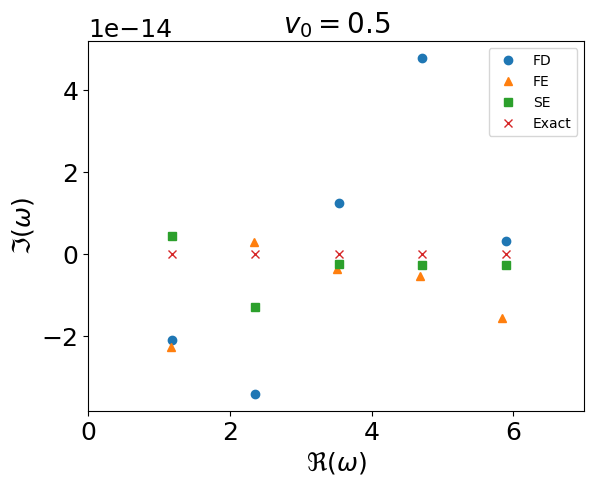
\includegraphics[width=\linewidth]{../../thesis/img/numerical-experiments/fixed-fixed/constant-v-v0=0.5}
		\caption{All modes are stable.}
	\end{subfigure}%
	\begin{subfigure}{0.5\textwidth}
		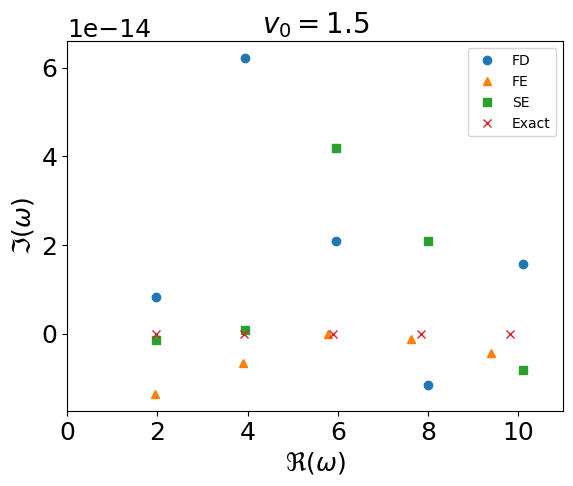
\includegraphics[width=\linewidth]{../../thesis/img/numerical-experiments/fixed-fixed/constant-v-v0=1.5}
		\caption{Filtered modes are stable.}
	\end{subfigure}
	\caption{Showing the first 5 eigenvalues of each method in each case. All methods are close to the exact eigenvalues.}
	\label{fig:constant-v-dirichlet}
\end{figure}

\subsection{Fixed-Open Boundary}
\begin{table} [H]
	\centering
	\caption{Relative error of each eigenvalue. Notice that the ground mode for subsonic case is non-zero.}
	\begin{tabular}{|c|c|c|c|c|c|}
		\hline
		$v_0=0.5$   & 0 & 1 & 2 & 3 & 4 \\
		\hline
		FD & 1.209e-05 & 3.458e-05 & 5.775e-05 & 8.153e-05 & 1.061e-04 \\
		\hline
		FE & 8.090e-05 & 2.007e-04 & 2.981e-04 & 6.596e-04 & 1.821e-03  \\
		\hline
	\end{tabular}
	\begin{tabular}{|c|c|c|c|c|c|}
		\hline
		$v_0=1.5$   & 1 & 2 & 3 & 4 & 5 \\
		\hline
		FD & 9.163e-05 & 2.435e-04 & 4.833e-04 & 8.160e-04 & 1.243e-03 \\
		\hline
		FE & 4.431e-04 & 7.924e-04 & 1.516e-03 & 3.103e-03 & 8.001e-03  \\
		\hline
	\end{tabular}
	\label{table:eigenvalue-error}
\end{table}

\begin{figure}[H]
	\centering
	\begin{subfigure}{0.5\textwidth}
		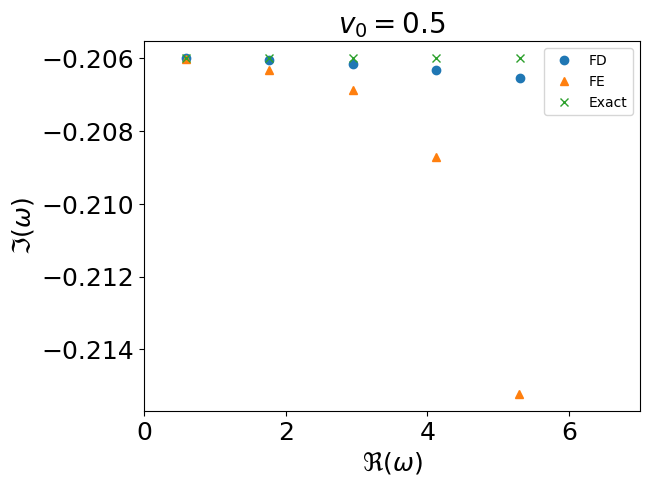
\includegraphics[width=\linewidth]{../../thesis/img/numerical-experiments/fixed-open/constant-v-v0=0.5}
		\caption{All modes are stable.}
	\end{subfigure}%
	\begin{subfigure}{0.5\textwidth}
		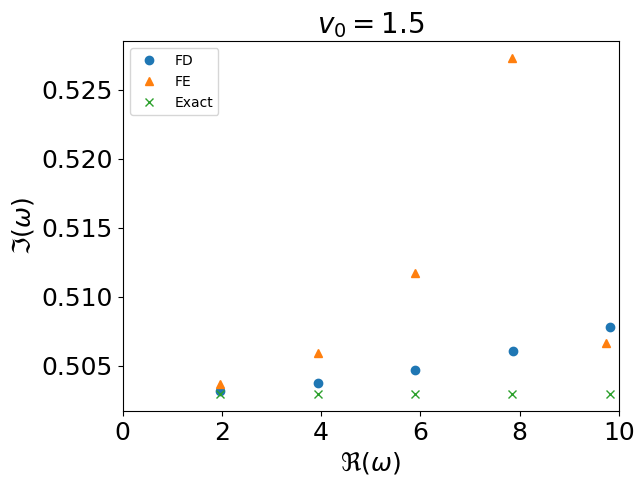
\includegraphics[width=\linewidth]{../../thesis/img/numerical-experiments/fixed-open/constant-v-v0=1.5}
		\caption{All modes are unstable.}
	\end{subfigure}
	\caption{Showing the first 5 eigenvalues of each method. Finite-difference method has much better accuracy than finite-element method.}
	\label{fig:constant-v-fixed-open}
\end{figure}


\section{Subsonic Case}
\subsection{Dirichlet Boundary}
When setting the mid-point velocity to be $M_m=0.5$, we have the subsonic velocity profile. This velocity profile is the orange line shown in Fig.\ref{fig:velocity-profiles}. With Dirichlet boundary condition, $\tilde{v}(\pm 1) =0$. The flow in magnetic nozzle is stable. Fig.\ref{fig:subsonic-v-dirichlet} shows the first few eigenvalues obtained by different discretizations. 

The order of growth rates obtained by different methods is $10^{-13}$, we can consider it to be stable.
\begin{figure} [H]
	\centering
	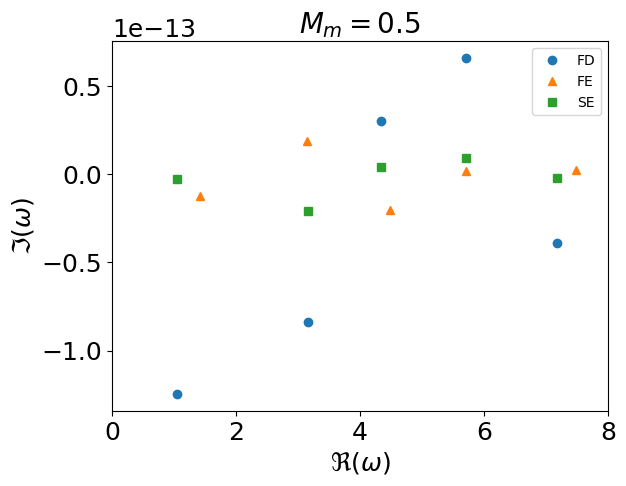
\includegraphics[width=0.7\linewidth]{../../thesis/img/numerical-experiments/fixed-fixed/subsonic-v}
	\caption{Showing the first 5 modes. It suggests that the flow in magnetic nozzle with subsonic velocity profile and Dirichlet boundary condition is stable.}
	\label{fig:subsonic-v-dirichlet}
\end{figure}

\subsection{Fixed-Open Boundary}
\begin{figure} [H]
	\centering
	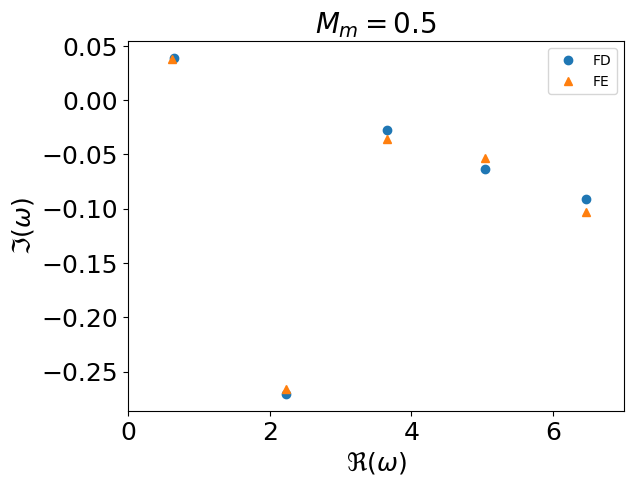
\includegraphics[width=0.7\linewidth]{../../thesis/img/numerical-experiments/fixed-open/subsonic-v}
	\caption{Showing the first 5 modes. The ground mode is unstable, other modes are stable.}
	\label{fig:subsonic-v-fixed_open}
\end{figure}


\section{Supersonic Case}
\subsection{Dirichlet Boundary}
When the velocity profile is supersonic, shown as purple line in Fig.\ref{fig:velocity-profiles}, spurious modes appeared as predicted in Chap.\ref{chap:theoretical-analysis}. Using the convergence test, we successfully eliminates all unstable modes. Fig.(\ref{fig:supersonic-v-dirichlet}) shows the first few filtered eigenvalues. As we can see the flow is stable.
\begin{figure} [H]
	\centering
	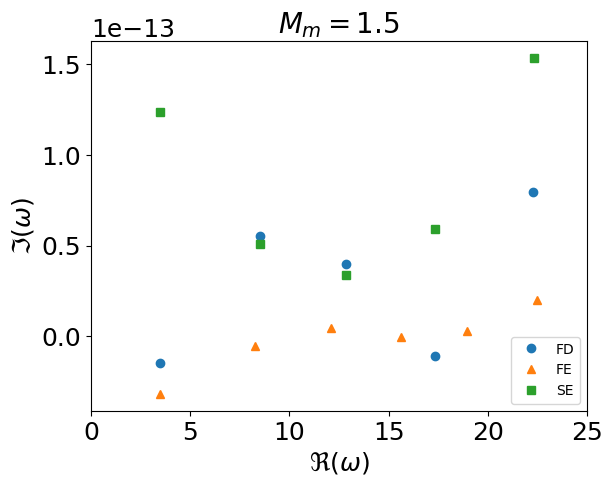
\includegraphics[width=0.7\linewidth]{../../thesis/img/numerical-experiments/fixed-fixed/supersonic-v}
	\caption{First few filtered eigenvalues are shown. The spurious modes are filtered by convergence test.}
	\label{fig:supersonic-v-dirichlet}
\end{figure}

\subsection{Fixed-Open Boundary}
\begin{figure} [H]
	\centering
	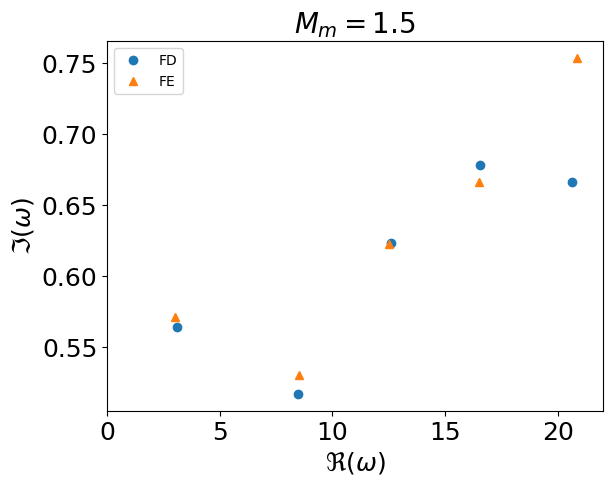
\includegraphics[width=0.7\linewidth]{../../thesis/img/numerical-experiments/fixed-open/supersonic-v}
	\caption{All modes are unstable.}
	\label{fig:supersonic-v-fixed-open}
\end{figure}


\section{Accelerating Case}
Starting from the singular point, we shoot the solution to the left boundary. We find the set of eigenvalues such that $\tilde{v}(-1)=0$. With these eigenvalues, we can extend the solution to the supersonic region $(0,1]$. The first five eigenvalues are drawn in the graph.
\begin{figure} [H]
	\centering
	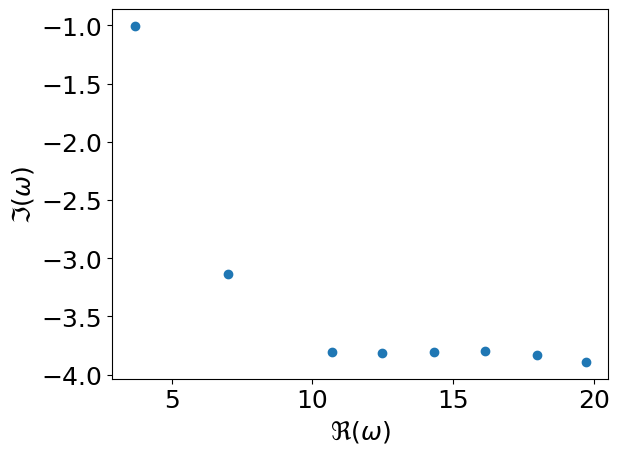
\includegraphics[width=0.7\linewidth]{../../thesis/img/numerical-experiments/accelerating-v}
	\caption{first five modes are stable.}
	\label{fig:accelerating-v}
\end{figure}

\chapter{conclusion}

\bibliographystyle{plain}
\bibliography{references} 

\chapter*{Appendix}
\section*{Lambert W function}


\section*{Verification of analytical solutions}
\begin{theorem}
    The general solution to 
    \[
        \omega^2\tilde{v} + 2i\omega\pdv{\tilde{v}}{z} + (1-v_0^2)\pdv[2]{\tilde{v}}{z} = 0
    \]
    is 
    \[ 
        \tilde{v} = \exp(-\frac{i\omega}{v_0+1})
        \left[ \exp(i\omega\frac{z+1}{v_0+1}) 
        - \exp(i\omega\frac{z+1}{v_0-1}) \right]
    \]
\end{theorem}
\begin{proof}
    The derivatives of $\tilde{v}$ are 
    \begin{align*}
        \tilde{v} &= \exp(-\frac{i\omega}{v_0+1})
        \left[ \exp(i\omega\frac{z+1}{v_0+1}) 
        - \exp(i\omega\frac{z+1}{v_0-1}) \right] \\
        \pdv{\tilde{v}}{z} &= i\omega\exp(-\frac{i\omega}{v_0+1})
        \left[ \frac{1}{v_0+1}\exp(i\omega\frac{z+1}{v_0+1}) - \frac{1}{v_0-1}\exp(i\omega\frac{z+1}{v_0-1}) \right] \\
        \pdv[2]{\tilde{v}}{z} &= -\omega^2\exp(-\frac{i\omega}{v_0+1})
        \left[ \frac{1}{(v_0+1)^2}\exp(i\omega\frac{z+1}{v_0+1}) - \frac{1}{(v_0-1)^2}\exp(i\omega\frac{z+1}{v_0-1}) \right]
    \end{align*}
    Then the rest is easy,
    \begin{align*}
        &\omega^2\tilde{v} + 2i\omega\pdv{\tilde{v}}{z} + (1-v_0^2)\pdv[2]{\tilde{v}}{z} \\
        =& \exp(-\frac{i\omega}{v_0+1})
            \left(1-\frac{2v_0}{v_0+1} + \frac{(1-v_0^2)}{(v_0+1)^2}\right)\exp(i\omega\frac{z+1}{v_0+1})
        \\
        &-\exp(-\frac{i\omega}{v_0+1})\left(1-\frac{2v_0}{v_0-1} + \frac{(1-v_0^2)}{(v_0-1)^2}\right)\exp(i\omega\frac{z+1}{v_0-1}) \\
        \\
        =& 0
    \end{align*}
\end{proof}

\begin{theorem}
    If $\omega = n\pi(1-v_0^2)/2$, then $\tilde{v}(\pm 1) = 0$.
\end{theorem}
\begin{proof}
    It is easy to see that $v(-1)=0$. As for $z=1$, we have
    \begin{align*}
        \tilde{v}(1) &\propto
        \exp(\frac{2i\omega}{v_0+1}) - \exp(\frac{2i\omega}{v_0-1}) \\
        &=
        \exp(in\pi(1-v_0)) - \exp(-in\pi(1+v_0)) \\
        &=
        (-1)^n\exp(-in\pi v_0) - (-1)^n\exp(-in\pi v_0) \\
        &= 0
    \end{align*}
\end{proof}

\begin{theorem}
    If 
    \[\omega = (v_0^2-1) \left[ \frac{n\pi}{2} - \frac{1}{4}i\ln\left(\frac{v_0-1}{v_0+1}\right) \right]\]
    then $\tilde{v}(-1) = 0$ and $\partial_z\tilde{v}(1) = 0$.
\end{theorem}
\begin{proof}
    It is easy to see that $v(-1)=0$. The derivative at $z=1$ is
    \begin{align*}
        \eval{\pdv{\tilde{v}}{z}}_{z=1} \propto&
        \frac{1}{v_0+1}\exp(\frac{2i\omega}{v_0+1}) - \frac{1}{v_0-1}\exp(\frac{2i\omega}{v_0-1}) \\
        =& \frac{1}{v_0+1}\exp(in\pi(v_0-1) + \frac{v_0-1}{2}\ln(\frac{v_0-1}{v_0+1})) \\
        &- \frac{1}{v_0-1}\exp(in\pi(v_0+1) + \frac{v_0+1}{2}\ln(\frac{v_0-1}{v_0+1})) \\
        =& \frac{(-1)^n}{v_0+1}\exp(in\pi v_0)\left(\frac{v_0-1}{v_0+1}\right)^{(v_0-1)/2} \\
        &- \frac{(-1)^n}{v_0-1}\exp(in\pi v_0)\left(\frac{v_0-1}{v_0+1}\right)^{(v_0+1)/2} \\
        =& 0
    \end{align*}
    The last equality holds because 
    \[ \frac{1}{v_0-1}\left(\frac{v_0-1}{v_0+1}\right)^{(v_0+1)/2} 
    = \frac{1}{v_0+1}\left(\frac{v_0-1}{v_0+1}\right)^{(v_0-1)/2}  \]
\end{proof}

\end{document}
